\chapter{Re\c{t}ele neuronale convolu\c{t}ionale}

Re\c{t}elele neuronale convolu\c{t}ionale  sunt foarte similare cu re\c{t}elele neuronale obi\c{s}nuite din capitolul anterior, ele sunt formate din neuroni care \^{i}nva\c{t}\u{a} \^{i}nt\u{a}riri \c{s}i bias-uri care s\u{a} \^{i}ndeplineasc\u{a} o anumit\u{a} sarcin\u{a}. Fiecare neuron prime\c{s}te date de intrare de la neuronii de pe nivelul inferiro lor, efectuaz\u{a} o opera\c{t}ie de multiplicare \^{i}ntre \^{i}nt\u{a}rir \c{s}i datele de intrare, adun\u{a} bias-ul la rezultatul ob\c{t}inut \^{i}n urma multiplic\u{a}rii iar dup\u{a} de cele mai multe ori aplic\u{a} o func\c{t}ie de activare, iar la final dup\u{a} ultimul nivel aplic\u{a}o func\c{t}ie de cost care s\u{a} determine c\^{a}t de aproape este re\c{t}eaua neuronal\u{a} de adevar \c{s}i dup\u{a} se aplic\u{a} propagarea \^{i}napoi pentru a actualiza \^{i}nt\u{a}ririle \c{s}i bias-ruile de pe fiecare nivel astfle \^{i}nc\^{a}t ca la urmatorul pas de \^{i}nv\u{a}\c{t}are a re\c{t}elei neuroanle aceasta s\u{a} ob\c{t}in\u{a} un rezultat mai mic de la func\c{t}ia de cost.

La prima vedere re\c{t}elele neuronale convolu\c{t}ionale seamana foarte mult cu re\c{t}elele neuronale obi\c{s}nuite, un lucru adevarat, \^{i}ns\u{a} exista unele diferen\c{t}e \^{i}ntre ele. Rec\c{t}elele neuronale convolutionale pleac\u{a} de la prezum\c{t}ia c\u{a} datele de intrare de pe primul nivel sunt imagini, fa\c{t}\u{a} de re\c{t}elele neuronale obi\c{s}nuite unde datele de intrare de pe primul nivel sunt ni\c{s}te vectori, din aceast\u{a} cauz\u{a} re\c{t}elele neuronale convolu\c{t}ionale se pot folosii de unele propiet\u{a}\c{t}i ale imaginilor asfel \^{i}nc\^{a}t acestea s\u{a} fiu mai eficiente in sarcini ce implica imaginile \c{s}i mai u\c{s}or de antrenat deoarece au nevoie de mai pu\c{t}ini parametrii dec\^{a}t ar avea nevoie o re\c{t}ea nuronale obi\c{s}nuit\u{a} \^{i}n \^{i}ndeplinirea aceleia\c{s}i sarcini.

\section{Arhitectura unei re\c{t}ele neuronale convolu\c{t}ionale}

Cum am v\u{a}zut in capitolul anterior, re\c{t}elele neuronale obi\c{s}nuite primesc ca date de intrare un  vector pe care \^{i}l trec prin mai multe nivele de neuroni, unde fiecare neuron de pe un nivel este conectat cu to\c{t}i neuronii de pe nivelul urm\u{a}tor \c{s}i cu to\c{t}i neuronii de pe nivelul inferior lui, \^{i}ns\u{a} nu este conectat cu neuronii de pe acela\c{s} nivel cu el. 

\par

Faptul c\u{a} re\c{t}elele neuronale convolu\c{t}ionale sunt concepute special pentru sarcini ce implic\u{a} imagini \c{s}i c\u{a} datele de intrare  au trei dimensiuni ( l\u{a}\c{t}ime, \^{i}n\u{a}l\c{t}ime \c{s}i ad\^{a}ncime ),  fa\c{t}\u{a} de re\c{t}elele neuronale obi\c{s}nuite unde datele de intrare au o singur\u{a} dimensiune, neuronii de pe nivele trebuiesc rearanja\c{t}i astfel \^{i}nc\^{a}t s\u{a} \^{i}ndeplineasc\u{a} c\^{a}t mai bine sarcina pe care o au de f\u{a}cut \c{s}i s\u{a} se folosesc\u{a} c\^{a}t mai bine de propriet\u{a}\c{t}ile pe care le au imaginile, din aceast\u{a} cauz\u{a} neuronii de pe un nivel la o re\c{t}ea neuronal\u{a} convolu\c{t}ional\u{a} sunt aranja\c{t}i pe trei dimensiuni ( l\u{a}\c{t}ime, \^{i}n\u{a}l\c{t}ime \c{s}i ad\^{a}ncime ), \^{i}n comapra\c{t}ie cu re\c{t}elele neuronale obi\c{s}nuite unde neuronii erau aranjati pe o singura dimensiune, cu acest timp de aranjament neuronii vor creea \^{i}nt\u{a}rir ce vor pune \^{i}n eviden\c{t}\u{a} anumite caracteristici ale unei imagine, caracteristici ce vor asigura o mai bun\u{a} performan\c{t}\u{a} a re\c{t}elei. Astfel c\u{a} un nivel dintr-o re\c{t}ea neuronal\u{a} convolu\c{t}ional\u{a} prime\c{s}te un volum de date cu trei dimensiuni \c{s}i produce un volum de date tot cu trei dimensiuni, volum de date care va fi dat mai departe la nivelul urm\u{a}tor lui.

\par 

\begin{center}
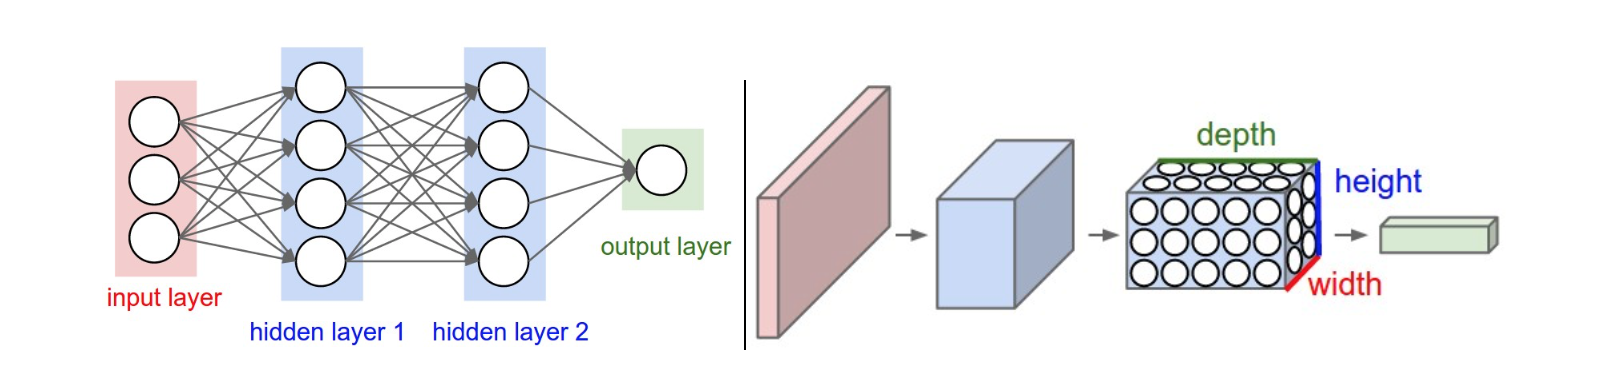
\includegraphics[width=450]{nn_cnn.png}
\end{center}

Imaginea de mai sus arat\u{a} diferen\c{t}a \^{i}ntre modul de aranjare a neuronilor pe o re\c{t}ea neuronal\u{a} obi\c{s}nuit\u{a} \c{s}i o re\c{t}ea neuronal\u{a} convolu\c{t}ional\u{a}.

\^{I}n re\c{t}elele neuronale convolu\c{t}ionale exit\u{a} trei tipuri de nivele, fa\c{t}\u{a} de re\c{t}elele neuronale obi\c{s}nuite unde exist\u{a} doar un singur tip, aceste nivele dintr-o re\c{t}ea neuronal\u{a} se numesc: nivelul convolu\c{t}ional, nivelul de pool \c{s}i nivelul conectat complet.

\subsection{Nivelul convolu\c{t}ional}

Nivelul convolu\c{t}ional este cel mai important nivel din cele trei \c{s}i cel care influen\c{t}eaz\u{a} cel mai mult deciziile re\c{t}elei neuronale. Acest nivel ca \c{s}i nivelele din re\c{t}elele neuronale are doi paramterii, \^{i}nt\u{a}ririle \c{s}i bias-urile, ins\u{a} \^{i}nt\u{a}ririle sunt organizate pe trei dimensiuni cum am discutat mai sus, astfle \^{i}nc\^{a}t acestea s\u{a} devina ni\c{s}te filtre care \^{i}n urma aplic\u{a}rii lor asupra datelor de intrare s\u{a} scoat\u{a} \^{i}n eviden\c{t}u unele detalii descriminatorii care s\u{a} ajute la indeplinirea sarcinii, \^{i}ns\u{a} bias-urile sunt la fel ca la neuronii din re\c{t}elele neuronale obi\c{s}nuite. 

\par

De cele mai multe ori \^{i}nt\u{a}ririle sunt mici \^{i}n \^{i}n\u{a}l\c{t}ime \c{s}i l\u{a}\c{t}ime dar sunt foarte mari in ad\^{a}ncime. [3x3x512] este un exemplu de dimensiune a unei \^{i}nt\u{a}riri, unde \^{i}n\u{a}\c{t}imea \c{s}i l\u{a}\c{t}imea au dimensiune 3 iar ad\^{a}ncimea are dimensiunea 512, motivul pentru care ad\^{a}ncimea este a\c{s}a de mare iar \^{i}n\u{a}l\c{t}imea \c{s}i l\u{a}\c{t}imea au dimensiuni a\c{s}a de mici  este pentru c\u{a} \^{i}n acest mod se pot construii mai multe filtre pe o por\c{t}iune mai mic\u{a} din datele de intrare \c{s}i, cum vom vedea in capitolele urm\u{a}toare, acest lucru faciliteaz\u{a} \^{i}n mod pozitiv acurate\c{t}ea re\c{t}elei neuronale.

\par

Nivelul convolu\c{t}ional gliseaz\u{a} o fereastr\u{a} de dimensiunea \^{i}nt\u{a}ririlor de-a lungul \c{s}i de-a latul datelor de intrare pornind de la col\c{t}ul de sus stanga a datelor de intrare \c{s}i face o \^{i}nmul\c{t}ire \^{i}ntre  datele de intrare aflate \^{i}n fereastr\u{a} \c{s}i cu \^{i}nt\u{a}ririle si  dup\u{a} la rezultat este adunat bias-ul. Acest proces este repetat p\^{a}n\u{a} c\^{a}nd fereastra ajunge in col\c{t}ul de jos dreapta a datelor de intrare. \^{I}n umra acestui proces va rezulta un volum de date bidimensional, dar acest procest este repetat pentru fiecare \^{i}nt\u{a}rire asftel c\u{a} la final vom avea un volum de date tridimensional. Cum am mai spus \c{s}i mai sus \^{i}nt\u{a}ririle \^{i}ntr-o re\c{t}ea neuronal\u{a} convolu\c{t}ional\u{a} sunt ni\c{s}te filtre care scot \^{i}n eviden\c{t}\u{a} anumte aspecte ale datelor de intrare, cum ar fi marginea unui obiect aflat \^{i}n imagine, o anumit\u{a} structur\u{a} care este caractersitic\u{a} unei anumite categorii de obiecte sau un patern.

\par

Pentru a se \^{i}n\c{t}elege mai bine cum func\c{t}ioneaz\u{a} nivelul convolu\c{t}ional s\u{a} presupunem c\u{a} avem o imagine de dimesniune [28x28x3] iar o \^{i}nt\u{a}rire are dimensiunea [5x5x3], a se observa faptul c\u{a} at\^{a}t  \^{i}nt\u{a}rirea c\^{a}t \c{s}i imaginea au aceea\c{s}i ad\^{a}ncime, respectiv 3, tot timpul ad\^{a}ncimea \^{i}nt\u{a}ririlr trebuie s\u{a} fie identic\u{a} cu cea a datelor de intrare pentru c\u{a} \^{i}n caz contrar nu s-ar putea face \^{i}nmul\c{t}irea \^{i}ntre datele de intrare \c{s}i \^{i}nt\u{a}riri, \^{i}ns\u{a} \^{i}n\u{a}l\c{t}imea si l\u{a}\c{t}imea \^{i}nt\u{a}ririlor trebuie s\u{a} fiu neap\u{a}rat mai mici dec\^{a}t a datelor de intrare altfle nu s-ar putea face glisarea. Dimensiunea \^{i}nt\u{a}ririlor \^{i}n \^{i}n\u{a}l\c{t}ime \c{s}i l\u{a}\c{t}ime este setat\u{a} manual, fiind un parametru important de setat \^{i}ntr-o re\c{t}ea neuronal\u{a} convolu\c{t}ional\u{a}. 

\begin{center}
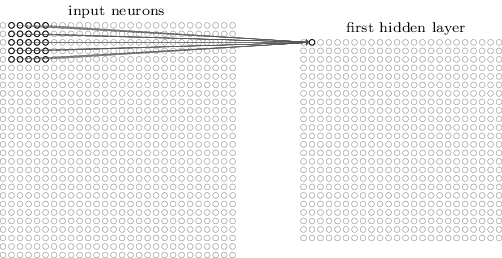
\includegraphics[width=300]{conv.png}
\end{center}

Cum se observ\u{a} \c{s}i \^{i}n imaginea de mai sus \^{i}n loc s\u{a} mai lu\u{a}m fiecare valoare a unui pixel separat \c{s}i s\u{a} o introducem \^{i}ntr-un neuron de pe un nivel intermediar ( hidden layer ) ca dat\u{a} de intrare putem s\u{a} grup\u{a}m pixelii in blocuri de pixeli \c{s}i s\u{a} \^{i}i trimitem grupa\c{t}i la un neuron de pe nivelul intermediar. \^{I}n cazul nostru vom face glisarea pe un grup de pixeli de dimensiunea [5x5x3] care va fi \^{i}nmul\c{t}it cu \^{i}nt\u{a}ririle noastre de dimensiune [5x5x3], \^{i}n umra rezultatului vom ob\c{t}ine o singur\u{a} valoare la care vom aduna bias-ul. Dac\u{a} se repeta procedeul  \c{s}i ne mi\c{s}c\u{a}m cu un pixel la dreapta sau in jos pentru fiecare bloc de pixeli pe care vrem s\u{a} \^{i}l extragem, atunci ca rezultat vom avea [24x24x1] de valori. Acum s\u{a} presupunem c\u{a} avem 32 de astfel de \^{i}nt\u{a}rir pe acest nivel \c{s}i reptet\u{a}m procedeul pentru fiecare, atunci ca rezultat final vom avea [24x24x32] de valori, valori care vor fi trimise mai departe c\u{a}tre urm\u{a}torul nivel. Un mare beneficiu al acestui mod de a grupa valorile \^{i}n blocuri de date mai mici peste care s\u{a} efectu\u{a}m opera\c{t}ia de \^{i}nmu\c{t}ire \c{s}i de adunare este c\u{a} se reduce semnificativ numarul de valori la o  \^{i}nt\u{a}riri de care am fi avut nevoie dac\u{a} am fi f\u{a}cut acela\c{s} lucru pentru toate datele dintr-o dat\u{a}, cum se face \^{i}ntr-o re\c{t}ea neuronal\u{a} obi\c{s}nuit\u{a}, spre exemplu \^{i}n cazul exemplificat mai sus avem nevoie doar de 5 x 5 x 3 = 75 de valori pentru o \^{i}nt\u{a}rire, \^{i}n cazul unei re\c{t}ele neuronale obi\c{s}nuite am fi avut nevoie de 28 x 28 x 3 = 2352 de valori pentru o \^{i}nt\u{a}rire. Prin reducerea numarului de valori de care avem nevoie pentru o \^{i}nt\u{a}rire vom cre\c{s}te viteza de \^{i}nv\u{a}\c{t}are a re\c{t}elei neuronale \c{s}i vom putea cre\c{s}te complexitatea acesteia.

\par

Mai sus am discutat despre cum nivelul convolu\c{t}ional transform\u{a} un volum de date tridimensional \^{i}ntr-un alt volum de date tridimensional \c{s}i cum \^{i}l calculeaz\u{a} pe acesta, \^{i}ns\u{a} nu am discutat cum se calculeaz\u{a} dimensiunea volumului de date tridimensional rezultat \^{i}n urma aplicarii nivelului convolu\c{t}ional peste  datele de intrare. Sunt trei parapetrii care controleaz\u{a} m\u{a}rimea datelor de ie\c{s}ire dintr-un nivel convolu\c{t}ional, acestea sunt: ad\^{a}ncimea, pasul de mi\c{s}care a ferestri c\^{a}nd se face glisarea ei peste volumul de date \c{s}i padding-ul. Ad\^{a}ncimea corespune numarului de \^{i}nt\u{a}riri pe care \^{i}l are respectivul nivel convolu\c{t}ional. Pasul este c\^{a}t de mult se mi\c{s}c\u{a} fereastra c\^{a}nd se face glisarea peste datele de intrare, dac\u{a} pasul este unu, atunci fereastra se va mi\c{s}ca la dreapta c\^{a}te un pixel iar c\^{a}nd va ajunge la cap\u{a}t va combor\^{a} un pixel \c{s}i va merge din noul la dreapta c\^{a}te un pixel p\^{a}n\u{a} la cap\u{a}, aces procedeu repet\^{a}nduse p\^{a}n\u{a} c\^{a}nd fereastra va ajunge \^{i}n col\c{t}ul de jos din dreapta. Dac\u{a} pasul este doi atunci fereastra se va mi\c{s}ca doi pixeli la dreapta \c{s}i \^{i}n jos, \^{i}ns\u{a} acest lucru va produce mai pu\c{t}ine date de ie\c{s}ire dec\^{a}t dac\u{a} pasul era unu. Padding-ul presupune numarul de r\^{a}nduri cu valoare zero pe care s\u{a} le punem \^{i}n jurul datelor de intrare astfel \^{i}nc\^{a}t s\u{a} putem controla dimensiunea datelor de ie\c{s}ire, spre exemplu cum aveam mai sus o imagine de dimesniune [28x28x3] \c{s}i \^{i}nt\u{a}riri de dimensiunea [5x5x3] \c{s}i un pas de unu aveam ca rezultat un volum de date de dimensiunea [24x24x1] pentru o \^{i}nt\u{a}rire, \^{i}ns\u{a} dac\u{a} ad\u{a}ug\u{a}m un padding de doi in jurul imaginii, atunci vom avea un volum de date de dimensiunea [32x32x3], deoarece padding-ul de doi s-a adugat jos, sus, la st\^{a}nga c\^{a}t \c{s}i la dreapta imaginii, iar \^{i}n urma aplic\u{a}rii nivelului convolu\c{t}ionale peste noul set de date vom avea un rezultat de dimensiunea [28x28x1]. Se observ\u{a} faptul c\u{a} noul rezultat are aceea\c{s}i dimensiune at\^{a}t pe \^{i}n\u{a}l\c{t}ime c\^{a}t \c{s}i pe l\u{a}\c{t}ime ca dimensiunea datelor ini\c{t}iale \^{i}nainte de aplicarea padding-ului, aces lucru  de a pastra dimensiunea datelor de ie\c{s}ire egal cu cel al datelor de intrare pe \^{i}n\u{a}l\c{t}ime \c{s}i l\u{a}\c{t}ime este foarte des folosit \^{i}n practic\u{a} deoarece prin acest fel se p\u{a}streaz\u{a} consisten\c{t}a datelor.

Putem s\u{a} exprim\u{a}m calculul volumului de ie\c{s}ire printr-o formul\u{a} foarte simpl\u{a} care arat\u{a} \^{i}n felul urm\u{a}tor:

$$ \frac{W - F + 2P }{S} + 1 $$

\^{I}n formula de mai sus W este marimea volumui de date, F este m\u{a}rimea ferestrei prin care se face glisarea peste date, S este pasul de mi\c{s}care a ferestre peste volumul de date iar P este padding-ul care se adauga \^{i}n jurlul volumului de date. Spre exemplu dac\u{a} avem un volum de date de dimensiune 7x7 \c{s}i int\u{a}riri de dimensiunea 3x3 cu un pas de 1 si un padding de 0 atunci vom avea un rezultat de dimensiunea 5x5, \^{i}ns\u{a} dac\u{a} cre\c{s}tem pasul la 2 atunci vom avea un rezultat de dimensiunea 3x3.

\subsection{Niveulul de pool}

Pooling layers: nivelul de pooling se pune intre doua nivele convolutionale pentru a se reduce cantitatea de informa\c{t}ie care se duce c\u{a}tre urm\u{a}torul nivel convolutional. Cel mai folosit tip de pooling este max-pooling care prime\c{s}te ca date de intrare valorile rezultate de la precedentul nivel convolutional \c{s}i le las\u{a} s\u{a} treac\u{a} doar pe cel cu valoarea cea mai mare catre urmatorul nivel convolutional ( vede\c{t}i imaginea de mai jos ), astfle c\u{a} acest nivel ne ajut\u{a} s\u{a} reducem cantitatea de date \c{s}i s\u{a} sc\u{a}p\u{a}m de datele nerelevante dintr-o re\c{t}ea convolutional\u{a}.

\begin{center}
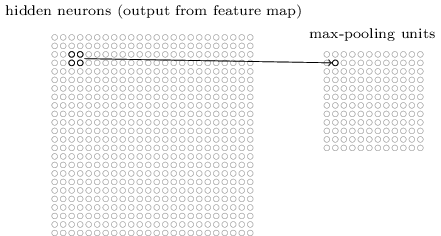
\includegraphics[width=300]{pool.png}
\end{center}

Cum se observ\u{a} \^{i}n imaginea de mai sus, nivelul de max-pooling prime\c{s}te patru valori de pe nivelul preceden \c{s}i las\u{a} o singur\u{a} valoarea s\u{a} treac\u{a} mai departe.